\chapter{Using Response and Writing Times to model Student Disengagement} \label{chap:engagementModel}

\section{Motivation}

In order to perform long term human-robot interactions in a educational context, it is important to know if the user is engaged on the task and if it is not, suggest an activity change. It is essential then, to have internal procedures that allow that. In \cite{joseph2005engagement} was established that time on task is an important predictor for how much students learn. Being also important that students are engaged during the learning process otherwise it will not be efficient. 

Therefore, we need to present a means for analyzing the response times and correctness of the student responses to model an overall level of engagement while using a computer tutor. This approach does not require humans to rate user interactions or measurements with biometric sensors since it can be measurable by statistical metrics. 

\section{Hypothesis}

Here, we hypothesize that a student who know how to write a shape would take less time to do it than someone who is not that skilled (who will take more to write the same shape). However, it is necessary to consider the children who wrote in a extremely short period of time. We can assume that students who spend less than a certain amount of time to write a shape are highly likely to be disengaged since they did not put time enough to write properly.

The fact that a user takes time to write a shape can not be taken as a sign of disengagement. So students who spent more time than a certain threshold are presumed to be just trying. Then, for purposes of building a model to predict a probability of disengagement, we consider only the regions R1, R2 and R3 present in figure \ref{fig:3pl}:

\vspace{5mm} %5mm vertical space

\begin{description}
  \item[Region 1] Performance at chance.
  \item[Region 2] Performance improve with time.
  \item[Region 3] Maximum of the performance
  \item[Region 4] Not considered
\end{description}

\begin{figure}[h!]
        \centering
        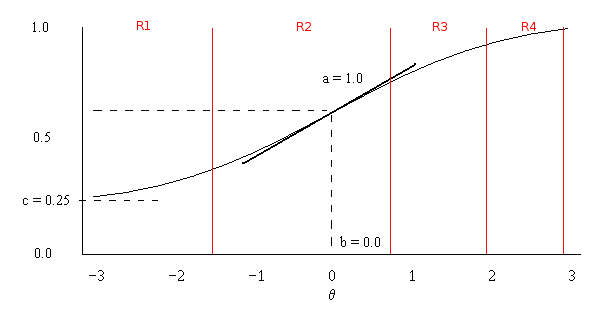
\includegraphics[width=0.6\textwidth]{figures/3PL.png}
        \caption{Three parameters logistic model from a item response function}
        \label{fig:3pl}
\end{figure}

The situation presented in figure \ref{fig:3pl} can be modeled by equation \ref{eq:itr}, the three parameter logistic (3PL) model which provides the probability of a correct response to a dichotomous item. In this equation the variable $\theta$ represents the student proficiency. The other three parameters control the shape of the logistic curve: \textit{a} is the discrimination which determines the steepness of the curve; and \textit{b} is the difficulty which controls the how much the curve is shifted from the axis center. Finally, \textit{c} is the guessing which sets the lower bound of the curve, in our case it is negligible since we assume the response can not be guessed blindly and still be correct.

\begin{equation}\label{eq:itr}
P(correct|\theta) = c + \frac{1-c}{1 + e^{-a(\theta-b)}}
\end{equation}

\section{Formal description time response-correctness }

Using Item Response Theory (IRT) \cite{embretson2013item} as starting point to model the relation between response time and engagement has used before in close questions assessment \cite{joseph2005engagement}. However, for shape writing follows a different procedure. In order to simplify the model we assume a dichotomy to assess if a shape is correct or not based on the distance to the reference shape introduced in chapter \ref{chap:correctness}.

However, the basic formula described in equation \ref{eq:itr} needs to evolve towards using a response time \textit{rt} as an input. In addition, discrimination and difficulty has to be calculated depending on the type of word used. For instance, to write a 3 characters word is not the same as writing a 5 characters one since takes a greater amount of time. It is also important to define an upper bound \textit{u} in the student's performance by a minimum distance to the reference shape that can be achieved. For instance, it is highly unlikely to obtain a correctness greater than 0.8.

The form of the new model is shown in equation \ref{eq:itr2}, where \textit{L} is the length of the word.

\begin{equation}\label{eq:itr2}
P(correct|rt,L) = \frac{u}{1 + e^{-a(-rt+b\cdot L)}}
\end{equation} 

In order to estimate \textit{a} and \textit{b} is necessary to do it separately for each length of word, since difficulty is highly accounted for that. Then, 3 character words are considered as \textit{easy}, 4 for \textit{moderate} and 5 for \textit{difficult}. For each model it is necessary to apply non-linear regression in order to obtain such unknowns. 

\section{Assessing correctness}
The model presented in figure \ref{fig:IRT} has been generated by collecting data from 10 adult people performing the writing of 5 different words with length $ L=3 $. Then, each of the letters of the same word was projected to the eigenspace and calculated its correctness (in terms of right or wrong setting a threshold) based on the distance to the reference letter. The mean of the three letters $ \bar{x} $ (see equation \ref{mean}) provides the result of a correct or incorrect word considering the condition shown in equation \ref{condition}.

\begin{equation}\label{mean}
 \bar{x}_{word} = \left ( \frac{1}{L}\cdot\sum_{i=1}^L{letter_i} \right )
\end{equation}

Then,

\begin{equation}\label{condition}
f(x)=\begin{cases}
 1, & \text{if $\bar{x}_{word} \geq 0.5$}.\\
 0, & \text{otherwise}.
\end{cases}
\end{equation}

where 1 and 0 are correct and incorrect word, respectively. As a final step, it is necessary to set the probability of a word to be correct given the response time. In order to do it, all samples have been grouped together by their writing response times in steps of 0.5 seconds, for instance two words written in 4.0 and 4.4 seconds would be grouped. Then, a mean criteria again was applied to decide the probability of being correct given a response time $P(correct|rt,L)$ comprise in the correspondent step (see green dots in figure \ref{fig:IRT}).

\begin{figure}[h!]
        \centering
        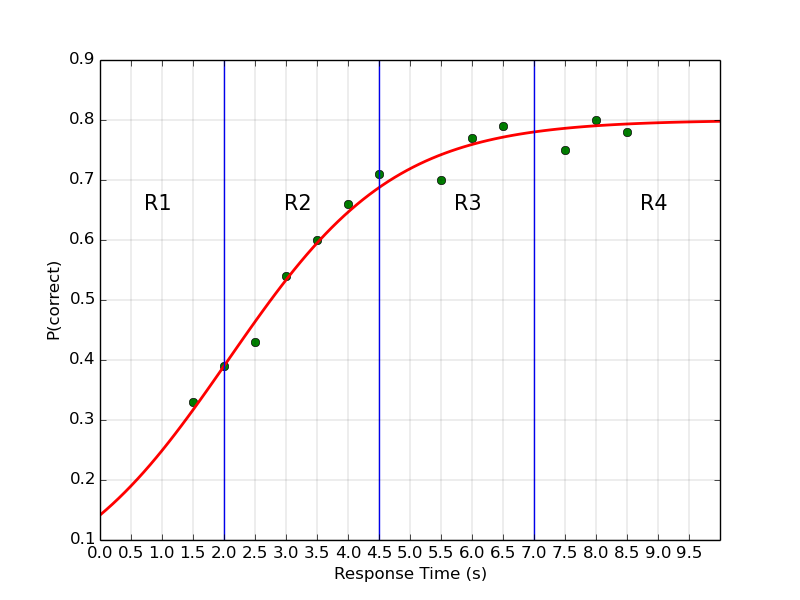
\includegraphics[width=0.6\textwidth]{figures/rt.png}
        \caption{Probability of being correct with respect to the response time}
        \label{fig:IRT}
\end{figure}

Finally, the results obtained for parameters \textit{a} and \textit{b} in a \textit{L=3} have been $ 0.7435 $ and $ 0.457 $ respectively.

\section{Disengagement estimation}
The current model can estimate the probability of a word to be correct given its writing time. However, to be able to calculate the engagement, it is necessary to assume that if a student is engaged, then he attempts to write the word with a maximum probability \textit{u} of being correct, which is the best performance in R3. This parameter is necessary since it is highly unlikely that the $ P(correct|rt,L) $ is higher than 0.8 and has been set based on a previous experiences. Therefore the model looks like in equation \ref{eq:irt3}

\begin{equation}\label{eq:irt3}
P_{disengaged} = \frac{u-P(correct|rt,L)}{u}
\end{equation}

For instance, someone who writes a word which has a length $ L=3 $ in a time $ rt=4 $ would obtain a $ P(correct|rt,L)= 0.67 $ so, $ P_{disengaged}=0.16 $ considering an upper bound $ u=0.8 $. And therefore, the probability of being engaged is $ P_{engaged}=1-0.16=0.84 $

\section{Limitations}
Despite generating a reasonable model, it presents some limitations. The main drawback of this method is the way to account for differences among students. But mainly, the model has not been tested so far, since the experiments carry out involved children around 5.5 years old and most of the time during the experiment they were trying to copy the shape models provided as helping material. Therefore, correctness and time responses were not obtained properly and were not suitable for the purpose of model training and testing.

In order to design a study were the present model can be tunned properly, it would be necessary to reproduce the experiments with 7 years old users with handwriting knowledge but with difficulties to perform it. In addition, it would be necessary to test the model to extract partial correlations between the disengagement measurements and learning gains after each iteration.  

